\hypertarget{gtkmenubutton-accelerators-font-pango-and-gsettings}{%
\section{GtkMenuButton, accelerators, font, pango and
gsettings}\label{gtkmenubutton-accelerators-font-pango-and-gsettings}}

Traditional menu structure is fine. However, buttons or menu items we
often use are not so many. Some mightn't be clicked at all. Therefore,
it's a good idea to put some frequently used buttons on the toolbar and
put the rest of the less frequently used operations into the menu. Such
menu are often connected to GtkMenuButton.

We will restructure tfe text file editor in this section. It will be
more practical. The buttons are changed to:

\begin{itemize}
\tightlist
\item
  Put open, save and close buttons to the toolbar. In addition,
  GtkMenuButton is added to the toolbar. This button shows a popup menu
  when clicked on. Here, popup means widely, including pull-down menu.
\item
  Put new, save as, preference and quit items to the menu under the menu
  button.
\end{itemize}

\hypertarget{signal-elements-in-ui-files}{%
\subsection{Signal elements in ui
files}\label{signal-elements-in-ui-files}}

The four buttons are included in the ui file
\passthrough{\lstinline!tfe.ui!}. The difference from prior sections is
signal tag. The following is extracted from
\passthrough{\lstinline!tfe.ui!} and it describes the open button.

\begin{lstlisting}[language=XML]
<object class="GtkButton" id="btno">
  <property name="label">Open</property>
  <signal name="clicked" handler="open_cb" swapped="TRUE" object="nb"></signal>
</object>
\end{lstlisting}

Signal tag specifies the name of the signal, handler and user\_data
object. They are the value of name, handler and object attributes.
Swapped attribute has the same meaning as
\passthrough{\lstinline!g\_signal\_connect\_swapped!} function. So, the
signal tag above works the same as the function below.

\begin{lstlisting}[language=C]
g_signal_connect_swapped (btno, "clicked", G_CALLBACK (open_cb), nb);
\end{lstlisting}

You need to compile the source file with ``-WI, --export-dynamic''
options. You can achieve this by adding ``export\_dynamic: true''
argument to executable function in
\passthrough{\lstinline!meson.build!}. And remove static class from the
handler.

\begin{lstlisting}[language=C]
void
open_cb (GtkNotebook *nb) {
  notebook_page_open (nb);
}
\end{lstlisting}

If you add static, the function is in the scope of the file and it can't
be seen from outside. Then the signal tag can't find the function.

\hypertarget{menu-and-gkmenubutton}{%
\subsection{Menu and GkMenuButton}\label{menu-and-gkmenubutton}}

Menus are described in \passthrough{\lstinline!menu.ui!} file.

\begin{lstlisting}[language=XML, numbers=left]
<?xml version="1.0" encoding="UTF-8"?>
<interface>
  <menu id="menu">
    <section>
      <item>
        <attribute name="label">New</attribute>
        <attribute name="action">win.new</attribute>
      </item>
      <item>
        <attribute name="label">Save As…</attribute>
        <attribute name="action">win.saveas</attribute>
      </item>
    </section>
    <section>
      <item>
        <attribute name="label">Preference</attribute>
        <attribute name="action">win.pref</attribute>
      </item>
    </section>
    <section>
      <item>
        <attribute name="label">Quit</attribute>
        <attribute name="action">win.close-all</attribute>
      </item>
    </section>
  </menu>
</interface>
\end{lstlisting}

There are four items, ``New'', ``Saveas'', ``Preference'' and ``Quit''.

\begin{itemize}
\tightlist
\item
  ``New'' menu creates a new empty page.
\item
  ``Saveas'' menu saves the current page as a new filename.
\item
  ``Preference'' menu sets preference items. This version of
  \passthrough{\lstinline!tfe!} has only font preference.
\item
  ``Quit'' menu quits the application.
\end{itemize}

These four menus are not used so often. That's why they are put to the
menu behind the menu button.

The menus and the menu button are connected with
\passthrough{\lstinline!gtk\_menu\_button\_set\_menu\_model!} function.
The variable \passthrough{\lstinline!btnm!} below points a GtkMenuButton
object.

\begin{lstlisting}[language=C]
  build = gtk_builder_new_from_resource ("/com/github/ToshioCP/tfe/menu.ui");
  menu = G_MENU_MODEL (gtk_builder_get_object (build, "menu"));
  gtk_menu_button_set_menu_model (btnm, menu);
\end{lstlisting}

\hypertarget{actions-and-accelerators}{%
\subsection{Actions and Accelerators}\label{actions-and-accelerators}}

Menus are connected to actions. Actions are defined with an array and
\passthrough{\lstinline!g\_action\_map\_add\_action\_entries!} function.

\begin{lstlisting}[language=C]
  const GActionEntry win_entries[] = {
    { "open", open_activated, NULL, NULL, NULL },
    { "save", save_activated, NULL, NULL, NULL },
    { "close", close_activated, NULL, NULL, NULL },
    { "new", new_activated, NULL, NULL, NULL },
    { "saveas", saveas_activated, NULL, NULL, NULL },
    { "pref", pref_activated, NULL, NULL, NULL },
    { "close-all", quit_activated, NULL, NULL, NULL }
  };
  g_action_map_add_action_entries (G_ACTION_MAP (win), win_entries, G_N_ELEMENTS (win_entries), nb);
\end{lstlisting}

There are seven actions, open, save, close, new, saveas, pref and
close-all. But there were only four menus. New, saveas, pref and
close-all actions correspond to new, saveas, preference and quit menu
respectively. The three actions open, save and close doesn't have
corresponding menus. Are thy necessary? These actions are defined
because of accelerators.

Accelerators are a kind of short cut key function. They are defined with
arrays and
\passthrough{\lstinline!gtk\_application\_set\_accels\_for\_action!}
function.

\begin{lstlisting}[language=C]
  struct {
    const char *action;
    const char *accels[2];
  } action_accels[] = {
    { "win.open", { "<Control>o", NULL } },
    { "win.save", { "<Control>s", NULL } },
    { "win.close", { "<Control>w", NULL } },
    { "win.new", { "<Control>n", NULL } },
    { "win.saveas", { "<Shift><Control>s", NULL } },
    { "win.close-all", { "<Control>q", NULL } },
  };

  for (i = 0; i < G_N_ELEMENTS(action_accels); i++)
    gtk_application_set_accels_for_action(GTK_APPLICATION(app), action_accels[i].action, action_accels[i].accels);
\end{lstlisting}

This code is a bit complicated. The array
\passthrough{\lstinline!action-accels[]!} is an array of structures. The
structure is:

\begin{lstlisting}[language=C]
  struct {
    const char *action;
    const char *accels[2];
  }
\end{lstlisting}

The member \passthrough{\lstinline!action!} is a string. The member
\passthrough{\lstinline!accels!} is an array of two strings. For
example,

\begin{lstlisting}[language=C]
{ "win.open", { "<Control>o", NULL } },
\end{lstlisting}

This is the first element of the array
\passthrough{\lstinline!action\_accels!}.

\begin{itemize}
\tightlist
\item
  The member \passthrough{\lstinline!action!} is ``win.open''. This
  specifies the action ``open'' belongs to the window object.
\item
  The member \passthrough{\lstinline!accels!} is an array of two
  strings, ``\textless Control\textgreater o'' and NULL. The first
  string specifies a key combination. Control key and `o'. If you keep
  pressing the control key and push `o' key, then it activates the
  action \passthrough{\lstinline!win.open!}. The second string NULL (or
  zero) means the end of the list (array). You can define more than one
  accelerator keys and the list must ends with NULL (zero). If you want
  to do so, the array length needs to be three or more. The parser
  recognizes ``\textless control\textgreater o'',
  ``\textless Shift\textgreater\textless Alt\textgreater F2'',
  ``\textless Ctrl\textgreater minus'' and so on. If you want to use
  symbol key like ``\textless Ctrl\textgreater-'', use
  ``\textless Ctrl\textgreater minus'' instead. Such relation between
  lower case and symbol (its character code) is specified in
  \href{https://gitlab.gnome.org/GNOME/gtk/-/blob/master/gdk/gdkkeysyms.h}{\passthrough{\lstinline!gdkkeysyms.h!}}
  in the Gtk4 source code.
\end{itemize}

\hypertarget{saveas-handler}{%
\subsection{Saveas handler}\label{saveas-handler}}

TfeTextView has already had a saveas function. So, only we need to write
is the wrapper function in \passthrough{\lstinline!tfenotebook.c!}.

\begin{lstlisting}[language=C, numbers=left]
static TfeTextView *
get_current_textview (GtkNotebook *nb) {
  int i;
  GtkWidget *scr;
  GtkWidget *tv;

  i = gtk_notebook_get_current_page (nb);
  scr = gtk_notebook_get_nth_page (nb, i);
  tv = gtk_scrolled_window_get_child (GTK_SCROLLED_WINDOW (scr));
  return TFE_TEXT_VIEW (tv);
}

void
notebook_page_saveas (GtkNotebook *nb) {
  g_return_if_fail(GTK_IS_NOTEBOOK (nb));

  TfeTextView *tv;

  tv = get_current_textview (nb);
  tfe_text_view_saveas (TFE_TEXT_VIEW (tv));
}
\end{lstlisting}

The function \passthrough{\lstinline!get\_current\_textview!} is the
same as before. The function
\passthrough{\lstinline!notebook\_page\_saveas!} simply calls
\passthrough{\lstinline!tfe\_text\_view\_saveas!}.

In \passthrough{\lstinline!tfeapplication.c!}, saveas handler just call
\passthrough{\lstinline!notebook\_page\_saveas!}.

\begin{lstlisting}[language=C, numbers=left]
static void
saveas_activated (GSimpleAction *action, GVariant *parameter, gpointer user_data) {
  GtkNotebook *nb = GTK_NOTEBOOK (user_data);
  notebook_page_saveas (nb);
}
\end{lstlisting}

\hypertarget{preference-and-alert-dialog}{%
\subsection{Preference and alert
dialog}\label{preference-and-alert-dialog}}

\hypertarget{preference-dialog}{%
\subsubsection{Preference dialog}\label{preference-dialog}}

Preference dialog xml definition is added to
\passthrough{\lstinline!tfe.ui!}.

\begin{lstlisting}[language=XML]
<object class="GtkDialog" id="pref">
  <property name="title">Preferences</property>
  <property name="resizable">FALSE</property>
  <property name="modal">TRUE</property>
  <property name="transient-for">win</property>
  <child internal-child="content_area">
    <object class="GtkBox" id="content_area">
      <child>
        <object class="GtkBox" id="pref_boxh">
          <property name="orientation">GTK_ORIENTATION_HORIZONTAL</property>
          <property name="spacing">12</property>
          <property name="margin-start">12</property>
          <property name="margin-end">12</property>
          <property name="margin-top">12</property>
          <property name="margin-bottom">12</property>
          <child>
            <object class="GtkLabel" id="fontlabel">
              <property name="label">Font:</property>
              <property name="xalign">1</property>
            </object>
          </child>
          <child>
            <object class="GtkFontButton" id="fontbtn">
            </object>
          </child>
        </object>
      </child>
    </object>
  </child>
</object>
\end{lstlisting}

\begin{itemize}
\tightlist
\item
  Preference dialog is an independent dialog. It is not a descendant
  widget of the top-level GtkApplicationwindow
  \passthrough{\lstinline!win!}. Therefore, There's no child tag that
  surrounds the dialog object.
\item
  There are four properties of the dialog. GtkDialog is a child object
  (not child widget) of GtkWindow, so it inherits all the properties
  from GtkWindow. Title, resizable, modal and transient-for properties
  are inherited from GtkWindow. Transient-for specifies a temporary
  parent window, which the dialog's location is based on.
\item
  internal-child attribute is used in the child tag above. GtkDialog has
  a GtkBox child widget. Its id is ``content\_area'' in
  \passthrough{\lstinline!gtkdialog.ui!}, which is the ui file of
  GtkDialog. (It is in the Gtk4 source files.) This box is provided for
  users to add content widgets in it. The tag
  \passthrough{\lstinline!<child internal-child="content\_area">!} is
  put at the top of the contents. Then you need to specify an object tag
  and define its class as GtkBox and its id as content\_area. This
  object is defined in \passthrough{\lstinline!gtkdialog.ui!} but you
  need to define it again in the child tag.
\item
  In the content area, defines GtkBox, GtkLabel and GtkFontButton.
\end{itemize}

I want the preference dialog to keep alive during the application lives.
So, it is necessary to catch ``close-request'' signal from the dialog
and stop the signal propagation. This is accomplished by returning TRUE
by the signal handler.

\begin{lstlisting}[language=C]
pref_close_cb (GtkDialog *pref, gpointer user_data) {
  return TRUE;
}

g_signal_connect (GTK_DIALOG (pref), "close-request", G_CALLBACK (pref_close_cb), NULL);
\end{lstlisting}

Generally, signal emission consists of five stages.

\begin{enumerate}
\def\labelenumi{\arabic{enumi}.}
\tightlist
\item
  Default handler is invoked if the signal's flag is
  \passthrough{\lstinline!G\_SIGNAL\_RUN\_FIRST!}. Default handler is
  set when a signal is registered. It is different from user signal
  handler, simply called signal handler, connected by
  \passthrough{\lstinline!g\_signal\_connect!}series function. Default
  handler can be invoked in either stage 1, 3 or 5. Most of the default
  handlers are \passthrough{\lstinline!G\_SIGNAL\_RUN\_FIRST!} or
  \passthrough{\lstinline!G\_SIGNAL\_RUN\_LAST!}.
\item
  Signal handlers are invoked, unless it is connected by
  \passthrough{\lstinline!g\_signal\_connect\_after!}.
\item
  Default handler is invoked if the signal's flag is
  \passthrough{\lstinline!G\_SIGNAL\_RUN\_LAST!}.
\item
  Signal handlers are invoked, if it is connected by
  \passthrough{\lstinline!g\_signal\_connect\_after!}.
\item
  Default handler is invoked if the signal's flag is
  \passthrough{\lstinline!G\_SIGNAL\_RUN\_CLEANUP!}.
\end{enumerate}

In the case of ``close-request'' signal, the default handler's flag is
\passthrough{\lstinline!G\_SIGNAL\_RUN\_LAST!}. The handler
\passthrough{\lstinline!pref\_close\_cb!} is not connected by
\passthrough{\lstinline!g\_signal\_connect\_after!}. So the number of
stages are two.

\begin{enumerate}
\def\labelenumi{\arabic{enumi}.}
\tightlist
\item
  Signal handler \passthrough{\lstinline!pref\_close\_cb!} is invoked.
\item
  Default handler is invoked.
\end{enumerate}

And If the user signal handler returns TRUE, then other handlers will be
stopped being invoked. Therefore, the program above prevents the
invocation of the default handler and stop the closing process of the
dialog.

The following codes are extracted from
\passthrough{\lstinline!tfeapplication.c!}.

\begin{lstlisting}[language=C]
static gulong pref_close_request_handler_id = 0;
static gulong alert_close_request_handler_id = 0;

... ...

static gboolean
dialog_close_cb (GtkDialog *dialog, gpointer user_data) {
  gtk_widget_hide (GTK_WIDGET (dialog));
  return TRUE;
}

... ...

static void
pref_activated (GSimpleAction *action, GVariant *parameter, gpointer nb) {
  gtk_widget_show (GTK_WIDGET (pref));
}

... ...

/* ----- quit application ----- */
void
tfe_application_quit (GtkWindow *win) {
  if (pref_close_request_handler_id > 0)
    g_signal_handler_disconnect (pref, pref_close_request_handler_id);
  if (alert_close_request_handler_id > 0)
    g_signal_handler_disconnect (alert, alert_close_request_handler_id);
  g_clear_object (&settings);
  gtk_window_destroy (GTK_WINDOW (alert));
  gtk_window_destroy (GTK_WINDOW (pref));
  gtk_window_destroy (win);
}

... ...

static void
tfe_startup (GApplication *application) {

  ... ...

  pref = GTK_DIALOG (gtk_builder_get_object (build, "pref"));
  pref_close_request_handler_id = g_signal_connect (GTK_DIALOG (pref), "close-request", G_CALLBACK (dialog_close_cb), NULL);

  ... ... 
}
\end{lstlisting}

The function \passthrough{\lstinline!tfe\_application\_quit!} destroys
top-level windows and quits the application. It first disconnects the
handlers from the signal ``close-request''.

\hypertarget{alert-dialog}{%
\subsubsection{Alert dialog}\label{alert-dialog}}

If a user closes a page which hasn't been saved, it is advisable to show
an alert to confirm it. Alert dialog is used in this application for
such a situation.

\begin{lstlisting}[language=XML]
  <object class="GtkDialog" id="alert">
    <property name="title">Are you sure?</property>
    <property name="resizable">FALSE</property>
    <property name="modal">TRUE</property>
    <property name="transient-for">win</property>
    <child internal-child="content_area">
      <object class="GtkBox">
        <child>
          <object class="GtkBox">
            <property name="orientation">GTK_ORIENTATION_HORIZONTAL</property>
            <property name="spacing">12</property>
            <property name="margin-start">12</property>
            <property name="margin-end">12</property>
            <property name="margin-top">12</property>
            <property name="margin-bottom">12</property>
            <child>
              <object class="GtkImage">
                <property name="icon-name">dialog-warning</property>
                <property name="icon-size">GTK_ICON_SIZE_LARGE</property>
              </object>
            </child>
            <child>
              <object class="GtkLabel" id="lb_alert">
              </object>
            </child>
          </object>
        </child>
      </object>
    </child>
    <child type="action">
      <object class="GtkButton" id="btn_cancel">
        <property name="label">Cancel</property>
      </object>
    </child>
    <child type="action">
      <object class="GtkButton" id="btn_accept">
        <property name="label">Close</property>
      </object>
    </child>
    <action-widgets>
      <action-widget response="cancel" default="true">btn_cancel</action-widget>
      <action-widget response="accept">btn_accept</action-widget>
    </action-widgets>
    <signal name="response" handler="alert_response_cb" swapped="NO" object="nb"></signal>
  </object>
\end{lstlisting}

This ui file describes the alert dialog. Some part are the same as
preference dialog. There are two objects in the content area, GtkImage
and GtkLabel.

GtkImage shows an image. The image can comes from files, resources, icon
theme and so on. The image above displays an icon from the current icon
theme. You can see icons in the theme by
\passthrough{\lstinline!gtk4-icon-browser!}.

\begin{lstlisting}
$ gtk4-icon-browser
\end{lstlisting}

The icon named ``dialog-warning'' is something like this.

\begin{figure}
\centering

\includegraphics[width=4.19cm,height=1.62cm]{../image/dialog_warning.png}
\caption{dialog-warning icon is like \ldots{}}
\end{figure}

These are made by my hand. The real image on the alert dialog is nicer.

The GtkLabel \passthrough{\lstinline!lb\_alert!} has no text yet. An
alert message will be inserted by the program later.

There are two child tags which have ``action'' type. They are button
objects located in the action area. Action-widgets tag describes the
actions of the buttons. \passthrough{\lstinline!btn\_cancel!} button
emits response signal with cancel response
(\passthrough{\lstinline!GTK\_RESPONSE\_CANCEL!}) if it is clicked on.
\passthrough{\lstinline!btn\_accept!} button emits response signal with
accept response (\passthrough{\lstinline!GTK\_RESPONSE\_ACCEPT!}) if it
is clicked on. The response signal is connected to
\passthrough{\lstinline!alert\_response\_cb!} handler.

The alert dialog keeps alive while the application lives. The
``close-request'' signal is stopped by the handler
\passthrough{\lstinline!dialog\_close\_cb!} like the preference dialog.

\hypertarget{close-and-quit-handlers}{%
\subsection{Close and quit handlers}\label{close-and-quit-handlers}}

If a user closes a page or quits the application without saving the
contents, the application alerts.

\begin{lstlisting}[language=C]
static gboolean is_quit;

... ...

void
close_cb (GtkNotebook *nb) {
  is_quit = false;
  if (has_saved (GTK_NOTEBOOK (nb)))
    notebook_page_close (GTK_NOTEBOOK (nb));
  else {
    gtk_label_set_text (lb_alert, "Contents aren't saved yet.\nAre you sure to close?");
    gtk_button_set_label (close_btn_close, "Close");
    gtk_widget_show (GTK_WIDGET (alert));
  }
}

... ...

static void
close_activated (GSimpleAction *action, GVariant *parameter, gpointer user_data) {
  GtkNotebook *nb = GTK_NOTEBOOK (user_data);
  close_cb (nb);
}

... ...

void
alert_response_cb (GtkDialog *alert, int response_id, gpointer user_data) {
  GtkNotebook *nb = GTK_NOTEBOOK (user_data);
  GtkWidget *win = gtk_widget_get_ancestor (GTK_WIDGET (nb), GTK_TYPE_WINDOW);

  gtk_widget_hide (GTK_WIDGET (alert));
  if (response_id == GTK_RESPONSE_ACCEPT) {
    if (is_quit)
      tfe_application_quit (GTK_WINDOW (win));
    else
      notebook_page_close (nb);
  }
}

static void
quit_activated (GSimpleAction *action, GVariant *parameter, gpointer user_data) {
  GtkNotebook *nb = GTK_NOTEBOOK (user_data);
  GtkWidget *win = gtk_widget_get_ancestor (GTK_WIDGET (nb), GTK_TYPE_WINDOW);

  is_quit = true;
  if (has_saved_all (nb))
    tfe_application_quit (GTK_WINDOW (win));
  else {
    gtk_label_set_text (lb_alert, "Contents aren't saved yet.\nAre you sure to quit?");
    gtk_button_set_label (btn_accept, "Quit");
    gtk_widget_show (GTK_WIDGET (alert));
  }
}

static void
tfe_startup (GApplication *application) {

  ... ...

  alert = GTK_DIALOG (gtk_builder_get_object (build, "alert"));
  alert_close_request_handler_id = g_signal_connect (GTK_DIALOG (alert), "close-request", G_CALLBACK (dialog_close_cb), NULL);
  lb_alert = GTK_LABEL (gtk_builder_get_object (build, "lb_alert"));
  btn_accept = GTK_BUTTON (gtk_builder_get_object (build, "btn_accept"));

  ... ...

}
\end{lstlisting}

The static variable \passthrough{\lstinline!is\_quit!} is true when user
tries to quit the application and false otherwise. When user presses
``Ctrl-w'', \passthrough{\lstinline!close\_activated!} handler is
invoked. It just calls \passthrough{\lstinline!close\_cb!}. When user
clicks on the close button, \passthrough{\lstinline!close\_cb!} handler
is invoked.

The handler sets \passthrough{\lstinline!is\_quit!} to false. The
function \passthrough{\lstinline!has\_saved!} returns true if the
current page has been saved. If it is true, it calls
\passthrough{\lstinline!notebook\_page\_close!} to close the current
page. Otherwise, it sets the message of the dialog and the label of the
button, then shows the alert dialog.

The response signal of the dialog is connected to the handler
\passthrough{\lstinline!alert\_response\_cb!}. It hides the dialog
first. Then checks the \passthrough{\lstinline!response\_id!}. If it is
\passthrough{\lstinline!GTK\_RESPONSE\_ACCEPT!}, which means user
clicked on the close button, then it closes the current page. Otherwise
it does nothing.

When user press ``Ctrl-q'' or clicked on the quit menu, then
\passthrough{\lstinline!quit\_activated!} handler is invoked. The
handler sets \passthrough{\lstinline!is\_quit!} to true. The function
\passthrough{\lstinline!has\_saved\_all!} returns true if all the pages
have been saved. If it is true, it calls
\passthrough{\lstinline!tfe\_application\_quit!} to quit the
application. Otherwise, it sets the message of the dialog and the label
of the button, then shows the alert dialog.

If the user clicked on the buttons on the alert dialog,
\passthrough{\lstinline!alert\_resoponse\_cb!} is invoked. It hides the
dialog and checks the \passthrough{\lstinline!response\_id!}. If it is
\passthrough{\lstinline!GTK\_RESPONSE\_ACCEPT!}, which means user
clicked on the quit button, then it calls
\passthrough{\lstinline!tfe\_application\_quit!} to quit the
application. Otherwise it does nothing.

The static variables \passthrough{\lstinline!alert!},
\passthrough{\lstinline!lb\_alert!} and
\passthrough{\lstinline!btn\_accept!} are set in the startup handler.
And the signal ``close-request'' and
\passthrough{\lstinline!dialog\_close\_cb!} handler are connected.

\begin{lstlisting}[language=C, numbers=left]
gboolean
has_saved (GtkNotebook *nb) {
  g_return_val_if_fail (GTK_IS_NOTEBOOK (nb), false);

  TfeTextView *tv;
  GtkTextBuffer *tb;

  tv = get_current_textview (nb);
  tb = gtk_text_view_get_buffer (GTK_TEXT_VIEW (tv));
  if (gtk_text_buffer_get_modified (tb))
    return false;
  else
    return true;
}

gboolean
has_saved_all (GtkNotebook *nb) {
  g_return_val_if_fail (GTK_IS_NOTEBOOK (nb), false);

  int i, n;
  GtkWidget *scr;
  GtkWidget *tv;
  GtkTextBuffer *tb;

  n = gtk_notebook_get_n_pages (nb);
  for (i = 0; i < n; ++i) {
    scr = gtk_notebook_get_nth_page (nb, i);
    tv = gtk_scrolled_window_get_child (GTK_SCROLLED_WINDOW (scr));
    tb = gtk_text_view_get_buffer (GTK_TEXT_VIEW (tv));
    if (gtk_text_buffer_get_modified (tb))
      return false;
  }
  return true;
}
\end{lstlisting}

\begin{itemize}
\tightlist
\item
  1-14: \passthrough{\lstinline!has\_saved!} function.
\item
  10: The function
  \passthrough{\lstinline!gtk\_text\_buffer\_get\_modified!} returns
  true if the content of the buffer has been modified since the modified
  flag had set false. The flag is set to false when:

  \begin{itemize}
  \tightlist
  \item
    the buffer is created.
  \item
    the contents of the buffer is replaced
  \item
    the contents of the buffer is saved to a file.
  \end{itemize}
\item
  11-13: This function returns true if the contents of the current page
  has been saved and no modification has been made. It returns false, if
  the current page has been modified and hasn't been saved.
\item
  16-33: \passthrough{\lstinline!has\_saved\_all!} function. This
  function is similar to \passthrough{\lstinline!has\_saved!} function.
  It returns true if all the pages have been saved. It returns false if
  at least one page has been modified since it last had been saved.
\end{itemize}

\hypertarget{notebook-page-tab}{%
\subsection{Notebook page tab}\label{notebook-page-tab}}

If you have some pages and edit them together, you might be confused
which file needs to be saved. Common file editors changes the tab when
the contents are modified. GtkTextBuffer provides ``modified-changed''
signal to notify the modification.

\begin{lstlisting}[language=C]
static void
notebook_page_build (GtkNotebook *nb, GtkWidget *tv, char *filename) {
  ... ...
  g_signal_connect (GTK_TEXT_VIEW (tv), "change-file", G_CALLBACK (file_changed_cb), NULL);
  g_signal_connect (tb, "modified-changed", G_CALLBACK (modified_changed_cb), tv);
}
\end{lstlisting}

When a page is built, connect ``change-file'' and ``modified-changed''
signals to \passthrough{\lstinline!file\_changed\_cb!} and
\passthrough{\lstinline!modified\_changed\_cb!} handlers respectively.

\begin{lstlisting}[language=C, numbers=left]
static void
file_changed_cb (TfeTextView *tv) {
  GtkWidget *nb =  gtk_widget_get_ancestor (GTK_WIDGET (tv), GTK_TYPE_NOTEBOOK);
  GtkWidget *scr;
  GtkWidget *label;
  GFile *file;
  char *filename;

  if (! GTK_IS_NOTEBOOK (nb)) /* tv not connected to nb yet */
    return;
  file = tfe_text_view_get_file (tv);
  scr = gtk_widget_get_parent (GTK_WIDGET (tv));
  if (G_IS_FILE (file)) {
    filename = g_file_get_basename (file);
    g_object_unref (file);
  } else
    filename = get_untitled ();
  label = gtk_label_new (filename);
  gtk_notebook_set_tab_label (GTK_NOTEBOOK (nb), scr, label);
}

static void
modified_changed_cb (GtkTextBuffer *tb, gpointer user_data) {
  TfeTextView *tv = TFE_TEXT_VIEW (user_data);
  GtkWidget *scr = gtk_widget_get_parent (GTK_WIDGET (tv));
  GtkWidget *nb =  gtk_widget_get_ancestor (GTK_WIDGET (tv), GTK_TYPE_NOTEBOOK);
  GtkWidget *label;
  const char *filename;
  char *text;

  if (! GTK_IS_NOTEBOOK (nb)) /* tv not connected to nb yet */
    return;
  else if (gtk_text_buffer_get_modified (tb)) {
    filename = gtk_notebook_get_tab_label_text (GTK_NOTEBOOK (nb), scr);
    text = g_strdup_printf ("*%s", filename);
    label = gtk_label_new (text);
    g_free (text);
    gtk_notebook_set_tab_label (GTK_NOTEBOOK (nb), scr, label);
  } else
    file_changed_cb (tv);
}
\end{lstlisting}

\begin{itemize}
\tightlist
\item
  1-20: \passthrough{\lstinline!file\_changed\_cb!} handler.
\item
  9-10: If the signal emits during the page is being built, it is
  possible that \passthrough{\lstinline!tv!} isn't a descendant of
  \passthrough{\lstinline!nb!}. That is, there's no page corresponds to
  \passthrough{\lstinline!tv!}. Then, it isn't necessary to change the
  name of the tab because no tab exists.
\item
  13-15: If \passthrough{\lstinline!file!} is GFile, then it gets the
  filename and unrefs \passthrough{\lstinline!file!}.
\item
  16-17: Otherwise, \passthrough{\lstinline!file!} is probably NULL and
  it assigns ``Untitled'' related name to
  \passthrough{\lstinline!filename!}
\item
  18-19: Creates GtkLabel with \passthrough{\lstinline!filename!} and
  sets the tab of the page with the GtkLabel.
\item
  22-41: \passthrough{\lstinline!modified\_changed\_cb!} handler.
\item
  31-32: If \passthrough{\lstinline!tv!} isn't a descendant of
  \passthrough{\lstinline!nb!}, then nothing needs to be done.
\item
  33-35: If the content is modified, then it gets the text of the tab
  and adds asterisk at the beginning of the text.
\item
  36-38: Sets the tab with the asterisk prepended text.
\item
  39-40: Otherwise the modified bit is off. It is because content is
  saved. It calls \passthrough{\lstinline!file\_changed\_cb!} and resets
  the filename, that means it leaves out the asterisk.
\end{itemize}

\hypertarget{font}{%
\subsection{Font}\label{font}}

\hypertarget{gtkfontbutton-and-gtkfontchooser}{%
\subsubsection{GtkFontButton and
GtkFontChooser}\label{gtkfontbutton-and-gtkfontchooser}}

The GtkFontButton is a button which displays the current font. It opens
a font chooser dialog if a user clicked on the button. A user can change
the font (family, style, weight and size) with the dialog. Then the
button keeps the new font and displays it.

The button and its signal ``font-set'' is initialized in the application
startup process.

\begin{lstlisting}[language=C]
static void
font_set_cb (GtkFontButton *fontbtn, gpointer user_data) {
  GtkWindow *win = GTK_WINDOW (user_data);
  PangoFontDescription *pango_font_desc;

  pango_font_desc = gtk_font_chooser_get_font_desc (GTK_FONT_CHOOSER (fontbtn));
  set_font_for_display_with_pango_font_desc (win, pango_font_desc);
}

static void
tfe_startup (GApplication *application) {

  ... ...

  fontbtn = GTK_FONT_BUTTON (gtk_builder_get_object (build, "fontbtn"));
  g_signal_connect (fontbtn, "font-set", G_CALLBACK (font_set_cb), win);

  ... ...

}
\end{lstlisting}

In the startup handler, set the variable
\passthrough{\lstinline!fontbtn!} to point the GtkFontButton object.
Then connect the ``font-set'' signal to
\passthrough{\lstinline!font\_set\_cb!} handler. The signal ``font-set''
is emitted when the user selects a font.

GtkFontChooser is an interface implemented by GtkFontButton. The
function \passthrough{\lstinline!gtk\_font\_chooser\_get\_font\_desc!}
gets the PangoFontDescription of the currently selected font.

Another function \passthrough{\lstinline!gtk\_font\_chooser\_get\_font!}
returns a font name which includes family, style, weight and size. I
thought it might be able to be applied to tfe editor. The font name can
be used to the \passthrough{\lstinline!font!} property of GtkTextTag as
it is. But it can't be used to the CSS without converting the string to
fit. CSS is appropriate to change the font of entire text in all the
buffers. I think GtkTextTag is less appropriate. If you know a good
solution, please post it to
\href{https://github.com/ToshioCP/Gtk4-tutorial/issues}{issue} and let
me know.

It takes many codes to set the CSS from the PangoFontDescription so the
task is left to the function
\passthrough{\lstinline!set\_font\_for\_display\_with\_pango\_font\_desc!}.

\hypertarget{css-and-pango}{%
\subsubsection{CSS and Pango}\label{css-and-pango}}

A new file \passthrough{\lstinline!css.c!} is made for functions related
to CSS.

\begin{lstlisting}[language=C, numbers=left]
#include "tfe.h"

void
set_css_for_display (GtkWindow *win, const char *css) {
  GdkDisplay *display;

  display = gtk_widget_get_display (GTK_WIDGET (win));
  GtkCssProvider *provider = gtk_css_provider_new ();
  gtk_css_provider_load_from_data (provider, css, -1);
  gtk_style_context_add_provider_for_display (display, GTK_STYLE_PROVIDER (provider), GTK_STYLE_PROVIDER_PRIORITY_USER);
}

void
set_font_for_display (GtkWindow *win, const char *fontfamily, const char *fontstyle, const char *fontweight, int fontsize) {
  char *textview_css;

  textview_css = g_strdup_printf ("textview {padding: 10px; font-family: \"%s\"; font-style: %s; font-weight: %s; font-size: %dpt;}",
                                      fontfamily, fontstyle, fontweight, fontsize);
  set_css_for_display (win, textview_css);
  g_free (textview_css);
} 

void
set_font_for_display_with_pango_font_desc (GtkWindow *win, PangoFontDescription *pango_font_desc) {
  PangoStyle pango_style;
  PangoWeight pango_weight; 
  const char *family;
  const char *style;
  const char *weight;
  int fontsize;

  family = pango_font_description_get_family (pango_font_desc);
  pango_style = pango_font_description_get_style (pango_font_desc);
  switch (pango_style) {
  case PANGO_STYLE_NORMAL:
    style = "normal";
    break;
  case PANGO_STYLE_ITALIC:
    style = "italic";
    break;
  case PANGO_STYLE_OBLIQUE:
    style = "oblique";
    break;
  default:
    style = "normal";
    break;
  }
  pango_weight = pango_font_description_get_weight (pango_font_desc);
  switch (pango_weight) {
  case PANGO_WEIGHT_THIN:
    weight = "100";
    break;
  case PANGO_WEIGHT_ULTRALIGHT:
    weight = "200";
    break;
  case PANGO_WEIGHT_LIGHT:
    weight = "300";
    break;
  case PANGO_WEIGHT_SEMILIGHT:
    weight = "350";
    break;
  case PANGO_WEIGHT_BOOK:
    weight = "380";
    break;
  case PANGO_WEIGHT_NORMAL:
    weight = "400"; /* or "normal" */
    break;
  case PANGO_WEIGHT_MEDIUM:
    weight = "500";
    break;
  case PANGO_WEIGHT_SEMIBOLD:
    weight = "600";
    break;
  case PANGO_WEIGHT_BOLD:
    weight = "700"; /* or "bold" */
    break;
  case PANGO_WEIGHT_ULTRABOLD:
    weight = "800";
    break;
  case PANGO_WEIGHT_HEAVY:
    weight = "900";
    break;
  case PANGO_WEIGHT_ULTRAHEAVY:
    weight = "900"; /* In PangoWeight definition, the weight is 1000. But CSS allows the weight below 900. */
    break;
  default:
    weight = "normal";
    break;
  }
  fontsize = pango_font_description_get_size (pango_font_desc) / PANGO_SCALE;
  set_font_for_display (win, family, style, weight, fontsize);
}
\end{lstlisting}

\begin{itemize}
\tightlist
\item
  3-11: \passthrough{\lstinline!set\_css\_for\_display!}. This function
  sets CSS for GdkDisplay. The content of the function is the same as
  the part of startup handler in the previous version of
  \passthrough{\lstinline!tfeapplication.c!}.
\item
  13-20: \passthrough{\lstinline!set\_font\_for\_display!}. This
  function sets CSS with font-family, font-style, font-weight and
  font-size.

  \begin{itemize}
  \tightlist
  \item
    font-family is a name of a font. For example, sans-serif, monospace,
    Helvetica and ``Noto Sans'' are font-family. It is recommended to
    quote font family names that contains white space, digits, or
    punctuation characters other than hyphens.
  \item
    font-style is one of normal, italic and oblique.
  \item
    font-weight specifies the thickness of a font. It is normal or bold.
    It can be specified with a number between 100 and 900. Normal is the
    same as 400. Bold is 700.
  \item
    font-size specifies the size of a font. Small, medium, large and
    12pt are font-size.
  \end{itemize}
\item
  17: Makes CSS text. The function
  \passthrough{\lstinline!g\_strdup\_printf!} creates a new string with
  printf-like formatting.
\item
  23-92:
  \passthrough{\lstinline!set\_font\_for\_display\_with\_pango\_font\_desc!}.
  This function takes out font-family, font-style, font-weight and
  font-size from the PangoFontDescription object and calls
  \passthrough{\lstinline!set\_font!}for\_display`.
\item
  32: Gets the font-family of
  \passthrough{\lstinline!pango\_font\_desc!}.
\item
  33-47: Gets the font-style of
  \passthrough{\lstinline!pango\_font\_desc!}. The functions
  \passthrough{\lstinline!pango\_font\_description\_get\_style!} returns
  an enumerated value.
\item
  48-89: Gets the font-weight of
  \passthrough{\lstinline!pango\_font\_desc!}. The function
  \passthrough{\lstinline!pango\_font\_description\_get\_weight!}
  returns an enumerated value. They corresponds to the numbers from 100
  to 900.
\item
  90: Gets the font-size of \passthrough{\lstinline!pango\_font\_desc!}.
  The function
  \passthrough{\lstinline!pango\_font\_description\_get\_size!} returns
  the size of a font. The unit of this size is (1/PANGO\_SCALE)pt. If
  the font size is 10pt, the function returns 10\emph{PANGO\_SCALE.
  PANGO\_SCALE is defined as 1024. Therefore, 10}PANGO\_SCALE is 10240.
\item
  91: calls \passthrough{\lstinline!set\_font\_for\_display!} to set CSS
  for the GdkDisplay.
\end{itemize}

For further information, see \href{https://docs.gtk.org/Pango/}{Pango
API Reference}.

\hypertarget{gsettings}{%
\subsection{GSettings}\label{gsettings}}

We want to maintain the font data after the application quits. There are
some ways to implement it.

\begin{itemize}
\tightlist
\item
  Make a configuration file. For example, a text file
  ``\textasciitilde/.config/tfe/font.cfg'' keeps font information.
\item
  Use GSettings object. The basic idea of GSettings are similar to
  configuration file. Configuration information data is put into a
  database file.
\end{itemize}

The coding with GSettings object is simple and easy. However, it is a
bit hard to understand the concept. This subsection describes the
concept first and then how to program it.

\hypertarget{gsettings-schema}{%
\subsubsection{GSettings schema}\label{gsettings-schema}}

GSettings schema describes a set of keys, value types and some other
information. GSettings object uses this schema and it writes/reads the
value of a key to/from the right place in the database.

\begin{itemize}
\tightlist
\item
  A schema has an id. The id must be unique. We often use the same
  string as application id, but schema id and application id are
  different. You can use different name from application id. Schema id
  is a string delimited by periods. For example,
  ``com.github.ToshioCP.tfe'' is a correct schema id.
\item
  A schema usually has a path. The path is a location in the database.
  Each key is stored under the path. For example, if a key
  \passthrough{\lstinline!font!} is defined with a path
  \passthrough{\lstinline!/com/github/ToshioCP/tfe/!}, the key's
  location in the database is
  \passthrough{\lstinline!/com/github/ToshioCP/tfe/font!}. Path is a
  string begins with and ends with a slash
  (\passthrough{\lstinline!/!}). And it is delimited by slashes.
\item
  GSettings save information as key-value style. Key is a string begins
  with lower case characters followed by lower case, digit or dash
  (\passthrough{\lstinline!-!}) and ends with lower case or digit. No
  consecutive dashes are allowed. Values can be any type. GSettings
  stores values as GVariant type, which may contain, for example,
  integer, double, boolean, string or complex types like an array. The
  type of values needs to be defined in the schema.
\item
  A default value needs to be set for each key.
\item
  A summery and description can be set for each key optionally.
\end{itemize}

Schemas are described in an XML format. For example,

\begin{lstlisting}[language=XML, numbers=left]
<?xml version="1.0" encoding="UTF-8"?>
<schemalist>
  <schema path="/com/github/ToshioCP/tfe/" id="com.github.ToshioCP.tfe">
    <key name="font" type="s">
      <default>'Monospace 12'</default>
      <summary>Font</summary>
      <description>The font to be used for textview.</description>
    </key>
  </schema>
</schemalist>
\end{lstlisting}

\begin{itemize}
\tightlist
\item
  4: The type attribute is ``s''. It is
  \href{https://docs.gtk.org/glib/struct.VariantType.html\#gvariant-type-strings}{GLib
  API Reference, GVariant Type Strings}. Other common types are:

  \begin{itemize}
  \tightlist
  \item
    ``b'': gboolean
  \item
    ``i'': gint32.
  \item
    ``d'': double.
  \end{itemize}
\end{itemize}

Further information is in
\href{https://docs.gtk.org/glib/struct.VariantType.html}{Glib API
Reference, VarientType}.

\hypertarget{gsettings-1}{%
\subsubsection{gsettings}\label{gsettings-1}}

First, let's try \passthrough{\lstinline!gsettings!} application. It is
a configuration tool for GSettings.

\begin{lstlisting}
$ gsettings help
Usage:
  gsettings --version
  gsettings [--schemadir SCHEMADIR] COMMAND [ARGS?]

Commands:
  help                      Show this information
  list-schemas              List installed schemas
  list-relocatable-schemas  List relocatable schemas
  list-keys                 List keys in a schema
  list-children             List children of a schema
  list-recursively          List keys and values, recursively
  range                     Queries the range of a key
  describe                  Queries the description of a key
  get                       Get the value of a key
  set                       Set the value of a key
  reset                     Reset the value of a key
  reset-recursively         Reset all values in a given schema
  writable                  Check if a key is writable
  monitor                   Watch for changes

Use "gsettings help COMMAND" to get detailed help.
\end{lstlisting}

List schemas.

\begin{lstlisting}
$ gsettings list-schemas
org.gnome.rhythmbox.podcast
ca.desrt.dconf-editor.Demo.Empty
org.gnome.gedit.preferences.ui
org.gnome.evolution-data-server.calendar
org.gnome.rhythmbox.plugins.generic-player

... ...
\end{lstlisting}

Each line is an id of a schema. Each schema has a key-value
configuration data. You can see them with list-recursively command.
Let's look at the keys and values of
\passthrough{\lstinline!org.gnome.calculator!} schema.

\begin{lstlisting}
$ gsettings list-recursively org.gnome.calculator
org.gnome.calculator source-currency ''
org.gnome.calculator source-units 'degree'
org.gnome.calculator button-mode 'basic'
org.gnome.calculator target-currency ''
org.gnome.calculator base 10
org.gnome.calculator angle-units 'degrees'
org.gnome.calculator word-size 64
org.gnome.calculator accuracy 9
org.gnome.calculator show-thousands false
org.gnome.calculator window-position (122, 77)
org.gnome.calculator refresh-interval 604800
org.gnome.calculator target-units 'radian'
org.gnome.calculator precision 2000
org.gnome.calculator number-format 'automatic'
org.gnome.calculator show-zeroes false
\end{lstlisting}

This schema is used by Gnome Calculator. Run the calculator and change
the mode, then check the schema again.

\begin{lstlisting}
$ gnome-calculator
\end{lstlisting}

\begin{figure}
\centering
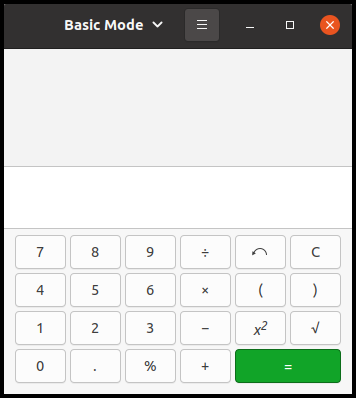
\includegraphics[width=5.34cm,height=5.97cm]{../image/gnome_calculator_basic.png}
\caption{gnome-calculator basic mode}
\end{figure}

Then, change the mode to advanced and quit.

\begin{figure}
\centering
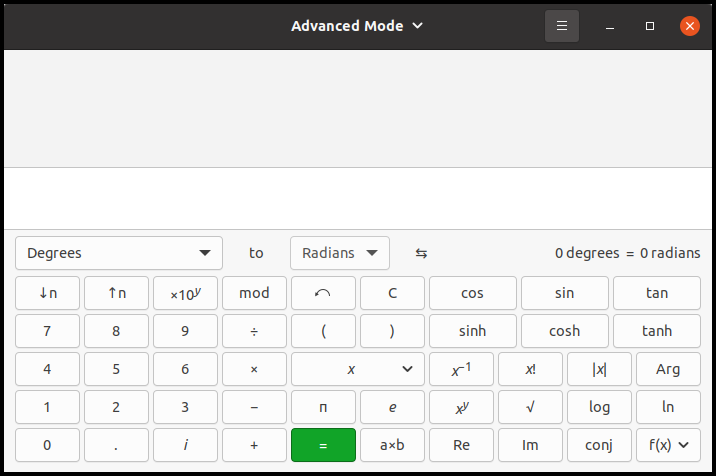
\includegraphics[width=10.74cm,height=7.14cm]{../image/gnome_calculator_advanced.png}
\caption{gnome-calculator advanced mode}
\end{figure}

Run gsettings and check whether the value of
\passthrough{\lstinline!button-mode!} changes.

\begin{lstlisting}
$ gsettings list-recursively org.gnome.calculator

... ...

org.gnome.calculator button-mode 'advanced'

... ...
\end{lstlisting}

Now we know that Gnome Calculator used gsettings and it has set
\passthrough{\lstinline!button-mode!} key to ``advanced''. The value
remains even the calculator quits. So when the calculator is run again,
it will appear as an advanced mode calculator.

\hypertarget{glib-compile-schemas}{%
\subsubsection{glib-compile-schemas}\label{glib-compile-schemas}}

GSettings schemas are specified with an XML format. The XML schema files
must have the filename extension \passthrough{\lstinline!.gschema.xml!}.
The following is the XML schema file for the application
\passthrough{\lstinline!tfe!}.

\begin{lstlisting}[language=XML, numbers=left]
<?xml version="1.0" encoding="UTF-8"?>
<schemalist>
  <schema path="/com/github/ToshioCP/tfe/" id="com.github.ToshioCP.tfe">
    <key name="font" type="s">
      <default>'Monospace 12'</default>
      <summary>Font</summary>
      <description>The font to be used for textview.</description>
    </key>
  </schema>
</schemalist>
\end{lstlisting}

The filename is ``com.github.ToshioCP.tfe.gschema.xml''. Schema XML
filenames are usually the schema id followed by ``.gschema.xml'' suffix.
You can use different name from schema id, but it is not recommended.

\begin{itemize}
\tightlist
\item
  2: The top level element is \passthrough{\lstinline!<schemalist>!}.
\item
  3: schema tag has \passthrough{\lstinline!path!} and
  \passthrough{\lstinline!id!} attributes. A path determines where the
  settings are stored in the conceptual global tree of settings. An id
  identifies the schema.
\item
  4: Key tag has two attributes. Name is the name of the key. Type is
  the type of the value of the key and specified with
  \href{https://docs.gtk.org/glib/struct.VariantType.html}{GLib API
  Reference, VariantType}.
\item
  5: default value of the key \passthrough{\lstinline!font!} is
  \passthrough{\lstinline!Monospace 12!}.
\item
  6: Summery and description elements describes the key. They are
  optional, but it is recommended to add them in the XML file.
\end{itemize}

The XML file is compiled by glib-compile-schemas. When compiling,
\passthrough{\lstinline!glib-compile-schemas!} compiles all the XML
files which have ``.gschema.xml'' file extension in the directory given
as an argument. It converts the XML file into a binary file
\passthrough{\lstinline!gschemas.compiled!}. Suppose the XML file above
is under \passthrough{\lstinline!tfe6!} directory.

\begin{lstlisting}
$ glib-compile-schemas tfe6
\end{lstlisting}

Then, \passthrough{\lstinline!gschemas.compiled!} is generated under
\passthrough{\lstinline!tfe6!}. When you test your application, set
\passthrough{\lstinline!GSETTINGS\_SCHEMA\_DIR!} so that GSettings objet
can find \passthrough{\lstinline!gschemas.compiled!}.

\begin{lstlisting}
$ GSETTINGS_SCHEMA_DIR=(the directory gschemas.compiled is located):$GSETTINGS_SCHEMA_DIR (your application name)
\end{lstlisting}

This is because GSettings object searches
\passthrough{\lstinline!GSETTINGS\_SCHEMA\_DIR!} for
\passthrough{\lstinline!gschemas.compiled!}.

GSettings object looks for this file by the following process.

\begin{itemize}
\tightlist
\item
  It searches \passthrough{\lstinline!glib-2.0/schemas!} subdirectories
  of all the directories specified in the environment variable
  \passthrough{\lstinline!XDG\_DATA\_DIRS!}. Most common directory is
  \passthrough{\lstinline!/usr/share/glib-2.0/schemas!}.
\item
  If \passthrough{\lstinline!GSETTINGS\_SCHEMA\_DIR!} environment
  variable is defined, it searches all the directories specified in the
  variable. \passthrough{\lstinline!GSETTINGS\_SCHEMA\_DIR!} can specify
  multiple directories delimited by colon (:).
\end{itemize}

In the directories above, all the \passthrough{\lstinline!.gschema.xml!}
files are stored. Therefore, when you install your application, follow
the instruction below to install your schemas.

\begin{enumerate}
\def\labelenumi{\arabic{enumi}.}
\tightlist
\item
  Make \passthrough{\lstinline!.gschema.xml!} file.
\item
  Copy it to one of the directories above. For example,
  \passthrough{\lstinline!/usr/local/share/glib-2.0/schemas!}.
\item
  Run \passthrough{\lstinline!glib-compile-schemas!} on the directory
  above.
\end{enumerate}

\hypertarget{meson.build}{%
\subsubsection{Meson.build}\label{meson.build}}

Meson provides \passthrough{\lstinline!gnome.compile\_schemas!} method
to compile XML file in the build directory. This is used to test the
application. Write the following to the
\passthrough{\lstinline!meson.build!} file.

\begin{lstlisting}
gnome.compile_schemas(build_by_default: true, depend_files: 'com.github.ToshioCP.tfe.gschema.xml')
\end{lstlisting}

\begin{itemize}
\tightlist
\item
  \passthrough{\lstinline!build\_by\_default!}: If it is true, the
  target will be build by default.
\item
  \passthrough{\lstinline!depend\_files!}: XML files to be compiled.
\end{itemize}

In the example above, this method runs
\passthrough{\lstinline!glib-compile-schemas!} to generate
\passthrough{\lstinline!gschemas.compiled!} from the XML file
\passthrough{\lstinline!com.github.ToshioCP.tfe.gschema.xml!}. The file
\passthrough{\lstinline!gschemas.compiled!} is located under the build
directory. If you run meson as \passthrough{\lstinline!meson \_build!}
and ninja as \passthrough{\lstinline!ninja -C \_build!}, then it is
under \passthrough{\lstinline!\_build!} directory.

After compilation, you can test your application like this:

\begin{lstlisting}
$ GSETTINGS_SCHEMA_DIR=_build:$GSETTINGS_SCHEMA_DIR _build/tfe
\end{lstlisting}

\hypertarget{gsettings-object-and-g_settings_bind}{%
\subsubsection{GSettings object and
g\_settings\_bind}\label{gsettings-object-and-g_settings_bind}}

Write gsettings related codes to `tfeapplication.c'.

\begin{lstlisting}[language=C]
... ...
static GSettings *settings;
... ...

void
tfe_application_quit (GtkWindow *win) {
  ... ...
  g_clear_object (&settings);
  ... ...
}

static void
tfe_startup (GApplication *application) {
  ... ...
  settings = g_settings_new ("com.github.ToshioCP.tfe");
  g_settings_bind (settings, "font", fontbtn, "font", G_SETTINGS_BIND_DEFAULT);
  ... ...
}
\end{lstlisting}

Static variable \passthrough{\lstinline!settings!} keeps a pointer to
GSettings instance. Before application quits, the application releases
the GSettings instance. The function
\passthrough{\lstinline!g\_clear\_object!} is used.

Startup handler creates GSettings instance with the schema id
``com.github.ToshioCP.tfe'' and assigns the pointer to
\passthrough{\lstinline!settings!}. The function
\passthrough{\lstinline!g\_settings\_bind!} connects the settings keys
(key and value) and the ``font'' property of
\passthrough{\lstinline!fontbtn!}. Then the two values will be always
the same. If one value changes then the other will automatically change.

You need to make an effort to understand GSettings concept, but coding
is very simple. Just create a GSettings object and bind it to a property
of an object.

\hypertarget{installation}{%
\subsection{Installation}\label{installation}}

It is a good idea to install your application in
\passthrough{\lstinline!$HOME/local/bin!} directory if you have
installed Gtk4 from the source (See Section 2). Then you need to put
\passthrough{\lstinline!--prefix=$HOME/local!} option to meson like
this.

\begin{lstlisting}
$ meson --prefix=$HOME/local _build
\end{lstlisting}

If you've installed Gtk4 from the distribution package,
\passthrough{\lstinline!--prefix!} option isn't necessary. You just
install \passthrough{\lstinline!tfe!} to the default bin directory like
\passthrough{\lstinline!/usr/local/bin!}.

Modify \passthrough{\lstinline!meson.build!} and add install option and
set it true in executable function.

\begin{lstlisting}
executable('tfe', sourcefiles, resources, dependencies: gtkdep, export_dynamic: true, install: true)
\end{lstlisting}

You can install your application by:

\begin{lstlisting}
$ ninja -C _build install
\end{lstlisting}

However, you need to do one more thing. Copy your XML file to
\passthrough{\lstinline!$HOME/local/share/glib-2.0/schemas/!}, which is
specified in \passthrough{\lstinline!GSETTINGS\_SCHEMA\_DIR!}
environment variable, and run
\passthrough{\lstinline!glib-compile-schemas!} on that directory.

\begin{lstlisting}
schema_dir = get_option('prefix') / get_option('datadir') / 'glib-2.0/schemas/'
install_data('com.github.ToshioCP.tfe.gschema.xml', install_dir: schema_dir)
\end{lstlisting}

\begin{itemize}
\tightlist
\item
  get\_option: This function returns the value of build options. The
  default value of the option `prefix' is ``/usr/local'', but it is
  ``\$HOME/local'' because we have run meson with prefix option. The
  default value of the option `datadir' is ``share''. The operator `/'
  connects the strings with `/' separator. So,
  \passthrough{\lstinline!$HOME/local/share/glib-2.0/schemas!} is
  assigned to the variable \passthrough{\lstinline!schema\_dir!}.
\item
  install\_data: This function installs the data to the install
  directory.
\end{itemize}

Meson can run a post compile script.

\begin{lstlisting}
meson.add_install_script('glib-compile-schemas', schema_dir)
\end{lstlisting}

This method runs `glib-compile-schemas' with an argument
\passthrough{\lstinline!schema\_dir!}. The following is
\passthrough{\lstinline!meson.build!}.

\begin{lstlisting}[numbers=left]
project('tfe', 'c')

gtkdep = dependency('gtk4')

gnome=import('gnome')
resources = gnome.compile_resources('resources','tfe.gresource.xml')
gnome.compile_schemas(build_by_default: true, depend_files: 'com.github.ToshioCP.tfe.gschema.xml')

sourcefiles=files('tfeapplication.c', 'tfenotebook.c', 'css.c', '../tfetextview/tfetextview.c')

executable('tfe', sourcefiles, resources, dependencies: gtkdep, export_dynamic: true, install: true)

schema_dir = get_option('prefix') / get_option('datadir') / 'glib-2.0/schemas/'
install_data('com.github.ToshioCP.tfe.gschema.xml', install_dir: schema_dir)
meson.add_install_script('glib-compile-schemas', schema_dir)
\end{lstlisting}

Source files of \passthrough{\lstinline!tfe!} is under src/tfe6
directory. Copy them to your temporary directory and try to compile and
install.

\begin{lstlisting}
$ meson --prefix=$HOME/local _build
$ ninja -C _build
$ GSETTINGS_SCHEMA_DIR=_build:$GSETTINGS_SCHEMA_DIR _build/tfe
$ ninja -C _build install
$ tfe
$ ls $HOME/local/bin
... ...
... tfe
... ...
$ ls $HOME/local/share/glib-2.0/schemas
com.github.ToshioCP.tfe.gschema.xml
gschema.dtd
gschemas.compiled
... ...
\end{lstlisting}

The screenshot is as follows.

\begin{figure}
\centering
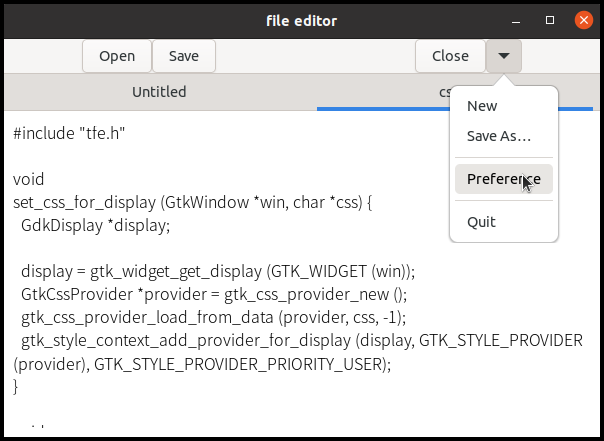
\includegraphics[width=9.06cm,height=6.615cm]{../image/tfe6.png}
\caption{tfe6}
\end{figure}
